\chapter{Introduction}
\textbf{RoboCup}, namely ``\textbf{Robot Soccer World Cup}'', is an annual international robotics competition which was founded in 1997. The aim of this game is to  promote robotics and AI research in a public appealing way. In 2016, it was held in Leipzig with more than 35,000 participants and teams from over 45 countries and regions. There are mainly four major categories in the whole RoboCup, namely \textit{RoboCup Soccer, RoboCup Home, RoboCup Rescue, RoboCup Industrial}. The original and still largest focus is the \textit{RoboCup Soccer}, in which teams of fully autonomous robots from different teams compete with each other. The teams are typically supported by a technical university or a research institute and carry strong academic and industrial backgrounds. \\
From the summer semester 2016, practical course ``Humanoid RoboCup'' was first offered at the Institute for Cognitive Systems. Each team consists of 3-4 master students with three NAO robots from Aldebaran Robotics as in \fref{NAOr}.\\
\begin{figure}[!htb]
    \centering
    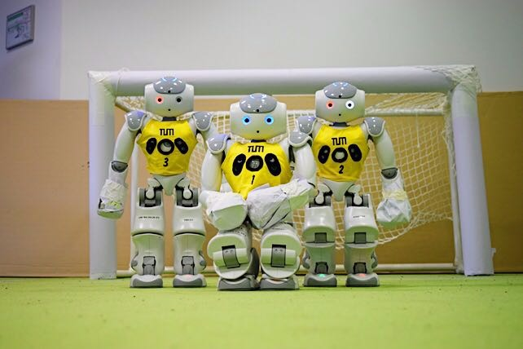
\includegraphics[width=0.6\textwidth]{pics/NAO}
    \caption{NAO robots}
    \label{NAOr}
\end{figure}
\clearpage
\section{Motivation}
The courses in artificial intelligence like machine learning, computer vision, pattern recognition are given as fundamental knowledge for the students in ``Kernbereich'' of Automation and robotics . After learning these theoretical knowledge, a practical course like ``Humanoid RoboCup'' is a perfect choice for students to know how these knowledge are applied in real scenarios. The given robots, namely NAOs, are cute from its out-looking and powerful with its computing ability.  Based on this platform, the students can choose their own tasks according to their different background knowledge.\\
Apart from technical knowledge, team-working, time-organization are also beneficial for the students involved in this course as they will work in small groups and decide when to work and how to work by groups.

\section{Overview and goals}
The course in winter semester of 2016/2017 is offered for the second time. It is divided into two phases, namely the lecture phase and practical phase. \\
In the lecture phase, about four lectures will be given as the introduction to different fields, such as control, vision, planning, or machine learning. In the second phase, the student will form individual teams for a soccer competition with NAOs, like yellow team or blue team. All the students in each team will do the basic setting up tasks together and then each student will choose his or her own task according to the on-hand knowledge. In this period, the student can come to the lecturers who given introductions in different field for more detailed help. \\
The goal of this semester is to establish the code framework and play a real robot game with each other. The code framework is developed based on the B-Human CodeRelease as in \cite{BHumanCodeRelease2015}. As the student from last semester only complete the match in simulation environments, more emphasis on real Robots were spent on testing and implementing designed algorithms.
\section{My Contributions}
Based on the problems found on real robots, the first task is to fix all these fundamental problems to make the robots be able to play a real game against another team.\\
The fundamental problems are discussed in detail in Chapter~\ref{Chap:Quick}, which includes:
\begin{itemize}
    \item Joint Calibration
    \item Camera and color Calibration
    \item Coding and Debugging in simulation
    \item Coding and Debugging on real robots
\end{itemize}
The insufficient calibration leads to some problems. To fix the problem of ``bad'' joint calibration, teammate Benno proposed a method called \textit{moving towards a target}. To get a better localization, teammate Ahmed proposed a method for better self-localization. For the details of these proposals one can refer to their reports. \\
Based on these proposals for fixing calibration problems, the behavior improvement is the main work of me and also the emphasis of this report. More concretely, the following new behaviors are proposed and implemented both in simulation and on real robots:
\begin{itemize}
    \item Defender: dynamic defense area
    \item Striker: dynamic kicking direction
\end{itemize}
These new behaviors are discussed in detail in Chapter~\ref{Chap:Imp}.
